%% Fall 2013 MDM Homework Template
\documentclass[12pt,letterpaper]{article}

\usepackage[utf8]{inputenc}
\usepackage[T1]{fontenc}
\usepackage{amsmath}
\usepackage{amsfonts}
\usepackage{amssymb}
\usepackage[left=2cm,right=2cm,top=2cm,bottom=2cm,headheight=22pt]{geometry}
\usepackage{fancyhdr}
\usepackage{setspace}
\usepackage{lastpage}
\usepackage{graphicx,subcaption}

\begin{document}

%other parameters
\setlength{\parskip}{1ex plus 0.5ex minus 0.2ex}
\setlength{\parindent}{0pt}

%header and footer parameters
\pagestyle{fancy}
\lhead{Math 1100}
\chead{Weekly Homework}
\rhead{Due: February 11}
\lfoot{}
\cfoot{\emph{Prof. Hitchman}}
\rfoot{}

\begin{center}
{
\Large
\textbf{Written Assignment \#4}
}
\end{center}

For each of the two knots below, say whether the knot is tricolorable or not. Explain how you know.

\begin{figure}[h]
    \centering
    \begin{subfigure}{.45\textwidth}
        \centering
        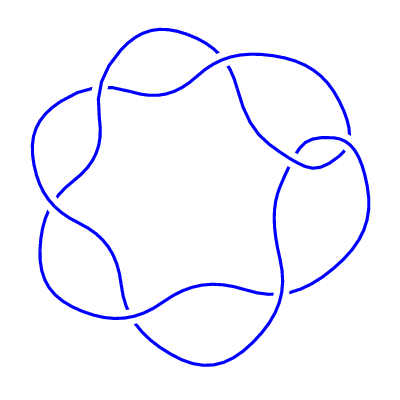
\includegraphics[width=\textwidth]{knotpics/7_2.png}
        \caption{Knot A}
    \end{subfigure}
    \qquad
    \begin{subfigure}{.45\textwidth}
        \centering
        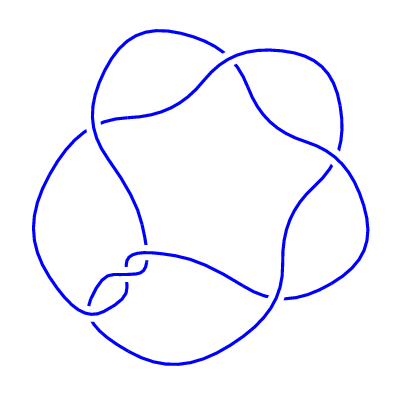
\includegraphics[width=\textwidth]{knotpics/7_3mirror.png}
        \caption{Knot B}
    \end{subfigure}
    \caption{Two knots with seven crossings}
\end{figure}





\end{document}
%sagemathcloud={"zoom_width":100}